\documentclass{article}
\usepackage{amsmath, amssymb}
\usepackage[utf8]{inputenc}
\usepackage[russian]{babel}
\usepackage{graphicx}

\title{Домашнее задание \\ \large Решения задач}
\author{AI Masters 25}
\date{}

\begin{document}

\maketitle

\section*{Задача 1}

\noindent \textbf{Решение:}\\
Оценка \(\hat{\alpha}\) несмещённая: \(E[\hat{\alpha}] = \alpha\).

Оценка эффективная когда ее дисперсия совпадает с нижней оценкой в неравенстве Крамера-Рао, которая
равна $1$ делить на информацию Фишера.
\begin{itemize}
  \item \textbf{Дисперсия:} \(D\left[\frac 1 n \sum\limits_{i=1}^{n} X_{i}\right] = \frac 1 {n^{2}}D\left[\sum\limits_{i=1}^{n}X_{1}\right] = \frac{\sigma^{2}}{n}\)
  \item \textbf{Информация Фишера:} Надо найти информацию Фишера одного наблюдения.
        \[I_{i}(\alpha) = E\left[\frac{\partial \ln{f(\alpha,X_{i})}}{\partial \alpha}\right],\]
        где \(f(\alpha, x) = \frac 1 {\sigma\sqrt{2\pi}}\exp\left(-\frac{{(x-\alpha)}^{2}}{2\sigma^{2}}\right)\).
        В итоге получаем \[I(\alpha) = nI_{i}(\alpha) = n E\left[\frac{{(X_{i}-\alpha)}^{2}}{\sigma^{4}}\right] =
        \frac n {\sigma^{2}}\]
\end{itemize}
Следовательно, \(\hat{\alpha}\) — эффективная оценка.

\section*{Задача 2}

\noindent \textbf{Решение:} \\
Оценка \(\hat{\sigma}^2\) несмещённая:
\[
E[\hat{\sigma}^2] = E\left[\frac{1}{n} \sum_{i=1}^n X_i^2\right] = \sigma^2.
\]
Аналогично предыдущей задаче ищем информацию Фишера и дисперсию.
\begin{itemize}
  \item \textbf{Информация Фишера:} для \(\sigma^2\) в \(N(0, \sigma^2)\):
\[
I(\sigma^2) = nI_{i}(\sigma^{2}).
\]
        Здесь \[I_{i}(\sigma^{2}) = E\left[\frac{\partial \ln{f(\sigma^{2},X_{i})}}{\partial \sigma^{2}}\right],\]
        где \(f(\sigma^{2}, x) = \frac 1 {\sqrt{2\pi\sigma^{2}}}\exp\left(-\frac{{(x-\alpha)}^{2}}{2\sigma^{2}}\right)\).\\
        Получаем \(I_{i}(\sigma) = \frac 1 {2\sigma^{4}}\).
        \[I(\sigma^{2}) = \frac{n}{2\sigma^{4}}\]
  \item \textbf{Дисперсия оценки}:
\[
        D\left[\frac{1}{n} \sum_{i=1}^n X_i^2\right] = \frac 1 {n} \left(E\left[X^{4}\right] - E^{2}\left[X^{2}\right]\right)
        = \frac{2\sigma^{4}}{n}.
\]
\end{itemize}
Таким образом, \(\hat{\sigma}^2\) — эффективная оценка.

\section*{Задача 3}

\noindent \textbf{Решение:} \\
Достаточная статистика для \(\theta\) — \(T = \max(X_1, ..., X_n)\). \\
Функция распределения расчитывается следующим образом:
\[
  P(\max(X_1, \ldots, X_n) < t) = P(X_{1} < t, \ldots, X_{n} < t) = \prod\limits_{i=1}^{n}P(X_{i}<t) = \frac{t^{n}}{\theta^{n}},
  0<t<\theta.
\]
Отсюда получаем вид для плотности распределения \(T\):
\[
f_T(t) = \frac{n t^{n-1}}{\theta^n}, \quad 0 \leq t \leq \theta.
\]
Найдем мат. ожидание $T$:
\[
E[T] = \int\limits_{0}^{\theta}\frac{n t^{n}}{\theta^n}dt = \frac{n}{n+1}\theta
\]
Оценка \(\hat{\theta} = \frac{n+1}{n} T\) является несмещённой:
\[
E[T] = \frac{n}{n+1} \theta \implies E[\hat{\theta}] = \theta.
\]
Так как \(T\) — полная и достаточная статистика, то \(\hat{\theta}\) — оптимальная оценка.

\section*{Задача 4}
\noindent \textbf{Решение:} \\
(a) Метод моментов: \\
$\overline{X} = \frac 1 n \sum\limits_{i=1}^{n}X_{i}$ --- оценка для $E[X]$ (первый момент).\\
$\overline{X^{2}} = \frac 1 n \sum\limits_{i=1}^{n}X_{i}^{2}$ --- оценка для $E\left[X^{2}\right]$(второй момент).

\[
\begin{cases}
  E[X_1] = \frac{a + b}2\\
  \widehat{E} = \overline{X}\\
  D[X_{1}] = \frac{{(b-a)}^{2}}{12}\\
  \widehat{D} = \overline{X^{2}} - \overline{X}^{2}
\end{cases}
\Rightarrow
\begin{cases}
  \frac{\hat{a} + \hat{b}}2 = \overline{X}\\
  \frac{\hat{b} - \hat{a}}2 = \sqrt{3\left(\overline{X^{2}} - \overline{X}^{2}\right)}
\end{cases}
\]
Отсюда получем оценки:
\[
  \begin{cases}
    \hat{a} = \overline{X} - \sqrt{3\left(\overline{X^{2}} - \overline{X}^{2}\right)}\\
    \hat{b} = \overline{X} + \sqrt{3\left(\overline{X^{2}} - \overline{X}^{2}\right)}
  \end{cases}
\]

(b) Пример кода на Python:
\begin{verbatim}
import numpy as np
import matplotlib.pyplot as plt

a_true, b_true = 1, 4
n_values = range(10, 1000, 10)
a_errors, b_errors = [], []

for n in n_values:
    sample = np.random.uniform(a_true, b_true, n)
    a_hat = np.mean(sample) - np.sqrt(3 * (np.var(sample)))
    b_hat = np.mean(sample) + np.sqrt(3 * (np.var(sample)))
    a_errors.append((a_hat - a_true)**2)
    b_errors.append((b_hat - b_true)**2)

plt.plot(n_values, a_errors, label='a_error')
plt.plot(n_values, b_errors, label='b_error')
plt.legend()
plt.show()
\end{verbatim}

\begin{figure}
    \centering
    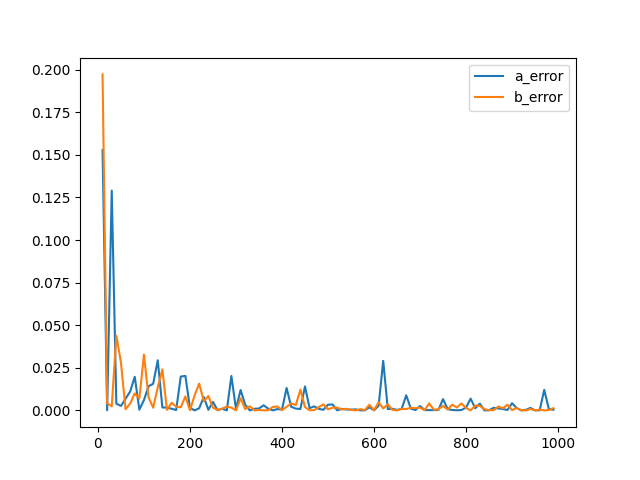
\includegraphics{plot.png}
    \caption{Результат работы}
\end{figure}

\section*{Задача 5}
\noindent \textbf{Решение:} \\
Функция правдоподобия:
\[
L(\alpha) = \prod\limits_{i=1}^{n}p(X_{i}) = \alpha^n \exp\left(\alpha \sum (X_i - \beta)\right).
\]
Логарифмируем:
\[
\ln L(\alpha) = n \ln \alpha + \alpha \sum (X_i - \beta).
\]
Условие максимума:
\[
\frac{d}{d\alpha} \ln L(\alpha) = \frac{n}{\alpha} + \sum (X_i - \beta) = 0 \implies \hat{\alpha} = -\frac{n}{\sum (X_i - \beta)}.
\]

\section*{Задача 6}
\noindent \textbf{Решение:} \\
Функция правдоподобия:
\[
L(\theta) = \prod_{i=1}^n \frac{1}{5} \cdot I_{\theta \leq X_i \leq \theta + 5}.
\]
Максимум достигается, когда все индикаторные функции равны \(1\). Таким образом:
\[
\hat{\theta} = \min(X_i) \quad \text{или} \quad \hat{\theta} = \max(X_i) - 5.
\]

\end{document}
